% Root File for a UC Dissertation / Thesis
% UCD thesis class: c/o Shwaine <shwaine@shwaine.com>
%
% modified by Dylan Beaudette, 2006,2010
% minor edits and source uploaded by Alex Mandel, 2010
% Source code available at http://github.com/wildintellect/ucdthesis
\documentclass[hidelinks,11pt,notableslist]{ucdthesis}
%\documentclass[10pt,twoside,final]{ucdthesis}
% \documentclass[10pt,twoside,draft]{ucdthesis}
% \documentclass[10pt,oneside,final]{ucdthesis}

% TODO: this makes strange things happen in the header...
% this is the version that grad studies wants
%\documentclass[11pt,oneside,final]{ucdthesis}

% when we are giving people drafts, use more of the page:
%\usepackage[letterpaper,left=0.75in,right=0.75in,top=1.25in,bottom=0.5in]{geometry}
\usepackage[paperwidth=8.5in,paperheight=11.0in,left=1.0in,right=01.0in,includefoot]{geometry}
% need this for the \foreach command
\usepackage{tikz}

% Turn on single spacing with \ssp.
% Turn on double spacing with \dsp.
% By default, your dissertation is double spaced, as is required by UCD.

% spacing in figures and tables and their captions can be
% changed here (\ssp for single-space, empty for same as surrounding
% text); for this to work, the command \figsp has to be included
% in every figure and table right after the \begin{figure}
\def\figsp{\ssp}
\def\figsp{}


% useful for drafts
% line numbers:
% http://www.ctan.org/tex-archive/help/Catalogue/entries/lineno.html
%
% \usepackage{lineno}

%
% SVN integration
%
\usepackage{svn-multi}

% customized headers
%
% http://www.ctan.org/tex-archive/help/Catalogue/entries/fancyhdr.html
\usepackage{fancyhdr}

% a better verbatim environment: c/o Pete Dirac
% use like this:
%\begin{Verbatim}[fontsize=8]
%	foobar
%\end{Verbatim}
\usepackage{fancyvrb}


% more flexible math support
\usepackage{amsmath}

% allow some pages to be landscape
\usepackage{lscape}

% more flexible definition of table environments
\usepackage{ctable}

%need this for \includegraphics{}
\usepackage{graphicx}

% TODO: use the new subfig package instead
% http://www.ctan.org/tex-archive/macros/latex/contrib/subfig/
%
%use this to put figures side by side
\usepackage{subfigure}

 % PDF links --- > breaks with some bibliography entries
\usepackage{hyperref}
% used for turning off floating
\usepackage{placeins}

% nice looking, parenthetical references
\usepackage[backend=biber, maxnames=5]{biblatex}
\addbibresource{main.bib}
%\usepackage[round]{natbib}

% fix nasty bug (usthesis + natbib)
% http://www.isi.edu/~johnh/SOFTWARE/uclathes.html
\def\newblock{\hskip .11em plus .33em minus .07em}

%make the index
\usepackage{makeidx}
\makeindex

% custom colors
\usepackage{color}
% make a color for comments
\definecolor{MyDarkBlue}{rgb}{0,0.08,0.45}

% customized captions with bold label and small, italic text
% table captions are located above tables
% http://www.kronto.org/thesis/tips/custom-captions.html
% http://www.ctan.org/tex-archive/macros/latex/contrib/caption/
% does this have any effect?
\usepackage{caption}
\renewcommand{\captionfont}{\small\itshape}
%
% modern method for setting up captions\
\captionsetup{margin=10pt,font=small,labelfont=bf}
%
% fix so that table captions have correct spacing
\captionsetup[table]{position=top}



% %
% %  fit more material on the page:
% %
%
% reset float-controlling parameters
\renewcommand{\floatpagefraction}{0.8}	% require fuller float pages

% N.B.: floatpagefraction MUST be less than topfraction !!
\renewcommand{\topfraction}{0.9}	% max fraction of floats at top
\renewcommand{\bottomfraction}{0.8}	% max fraction of floats at bottom
\newcommand{\toolname}{Pyandrazzi}




%%% Document Portion:
\begin{document}


%
%% Title, Front Matter, and Abstract:
% Declarations for Front Matter

% MS Thesis = 0, Phd Dissertation = 1
\isdissertation{0}

% electronic submission? Paper only = 0, Electronic = 1
\iselectronic{0}

\title{Quantifying the Effects of Permission Removal from Android Applications}
\author{Kristen M. Kennedy}

\degreemonth{December}
\degreeyear{2013}
\degree{Master of Science}

%\committee{Chen-Nee Chuah \Hao Chen and \Mathew Bishop}
\chaira{Chen-Nee Chuah}
\chairb{Hao Chen}
\othermembers{Mathew Bishop\\}
\numberofmembers{3}

\prevdegrees{B.E,M.E (Catholic University of America)}

\field{Electical and Computer Engineering}
\campus{Davis}


% add the abstract here

% Their are two abstracts. One that is published externally from your
% dissertation, and one that is internal. Of course, the text of the
% abstract will be the same. So, we define a macro to hold the body of our
% abstract.

% at 345 words
\newcommand{\myabstract}{
With the growing popularity of Android smart phones, it is increasingly important to ensure the security of sensitive user information.  A recent study found that approximately 26\% of Android applications in Google Play can access personal data, such as contacts and email, and 42 percent, GPS location data~\cite{Higgins}.  While Android is known for giving the user control, it falls short when it comes to enabling and disabling the permissions on applications.  Currently, the user is given the option to either give the application every permission it desires or not install it.  While researchers have proposed approaches for allowing users to modify the permissions granted to applications, it is unclear how removing permissions would affect the behavior of current applications.  At present, developers expect all requested permissions to be granted.  

This study takes the first step towards quantifying the impact of enabling users to statically remove permissions on Android applications post-installation.  An automated testing system, \toolname, was developed and customized for evaluating the effect of removing individual permissions from applications.  Using \toolname, the effects of removing 7 common permissions were evaluated using sets of randomly selected applications that request them.  It was determined that approximately 5.  8\% of the 700 applications tested crash after a permission is removed and that the removal of certain permissions is handled more gracefully than others.  The results of this study will help users make more informed decisions when removing permissions and help developers make their applications more robust to permission revocation.  
}



% Here is the first, external, abstract.
%\begin{abstract}
%	\myabstract
%	\abstractsignature
%\end{abstract}

\begin{frontmatter}
\maketitle

% A copyright page is optional. If you have one, it must immediately
% follow the title page. For more information about the copyright page
% see the UCD's Office of Graduate Studies web site.
\copyrightpage


% Here is the second, internal, abstract.
% Update: Melissa Danforth 2006
% Inline abstract is now part of front matter according to coordinator
\newpage
   \begin{inlineabstract}
	\addcontentsline{toc}{chapter}{\abstractname}
	\begin{small}
	\myabstract
	\end{small}
		
	% DEB 2010/07/09
	% don't really need the signature for the in-line abstract
	% \abstractsignature
   \end{inlineabstract}
\begin{acknowledgments}
xxxxxxx
\end{acknowledgments}    

% dedication 
%\begin{dedication}
%\null\vfil
%{\large
%\begin{center}
%xxxx
%\end{center}}
%\vfil\null
%\end{dedication}



\tableofcontents
\listoffigures
\begingroup
\let\clearpage\relax
\listoftables
\endgroup
%\listoffigures
%\listoftables



\end{frontmatter}

%\setlength{\footskip}{10pt}
%
% the chapters
%

% set page style:
% make the chapter and section smaller, chapter and section numbers are removed
% fancyplain will keep the page numbers at the bottom of all pages
%\pagestyle{fancy} %Note the \fancyplain command !!!
%\fancyhf{} 
%\fancyhead[R]{\thepage} 
%\fancypagestyle{plain}
%\fancyhf{}
\pagestyle{plain}
\pagenumbering{arabic}
\renewcommand{\chaptermark}[1]{\markboth{\small{#1}}{}}
\renewcommand{\sectionmark}[1]{\markright{\small{#1}}{}}


% TODO: this is only for draft copies !!
% start line number printing
%
%\linenumbers


% chapter 1
%This is an example for a chapter, additional chapter can be added in the skeleton-thesis
%To generate the final document run latex, build and quick build commands on the skeleton-thesis file not this one.
\chapter{Introduction}
Android is by far the most popular smartphone operating system at the time of this writing. With around 75\% of the global smartphone market~\cite{Perez}, its application ecosystem has grown along with it.  According to a recent Google press release, Google Play now has around 700,000 applications~\cite{Womack}. Unlike the Apple iOS ecosystem whose applications are centrally verified before becoming available, Android applications are more lightly vetted. This puts more responsibility on the user to make the important decision of which applications they trust. The permissions architecture employed by Android, however, makes these trust decisions more difficult. 

\subsection{Mobile Device Permission Models}
In the current implementation, application developers are responsible for defining the set of permissions their application asks for independent of what their application’s code actually uses~\cite{Felt}. The list is presented to the user at install-time whether installing an 
application obtained through the Google Play market or elsewhere. This list contains the canonical names given to each permission object, but provides little context as to what the permission is being used for. In the latest API, Google has added more description and added warning levels . At the end of the day, however, users have no choice but to accept the permissions list as presented to them, or not install the application.

While all smartphone applications are susceptible to being over permissioned, Apple's iOS and Blackberry's OS both give the user the ability to revoke an applications permissions. iOS uses a "dynamic" permissions model; the user is prompted once per application to use phone features such as the GPS receiver. The user then has the option of changing their decision through the system's settings menu. 

Blackberry OS uses a "static" approach similar to that of Android. Application developers declare the set of permissions they would like their program to have, and this list is presented to the user at installation. However, unlike Android, the user has the option to edit the list and revoke any permission. This approach adds a degree of granularity to an otherwise binary trust decision and is the approach explored in this study.

\subsection{Removing Permissions from Android Apps}

Shown in Figure~\ref{fig:permission}, is the application permissions listing for a Flashlight application obtained through the Play market.  While one could reason this application would only need the hardware controls necessary to turn on the phone's light, due to the large quantities of ad network libraries and other debris embedded within, it asks for much more. If permissions were editable, the user would be able to trust this application’s ability to operate the flashlight only, and not have to worry about the true reason for the other permission requests.

\begin{figure}[t]
\centerline{\resizebox{0.4\linewidth}{!}{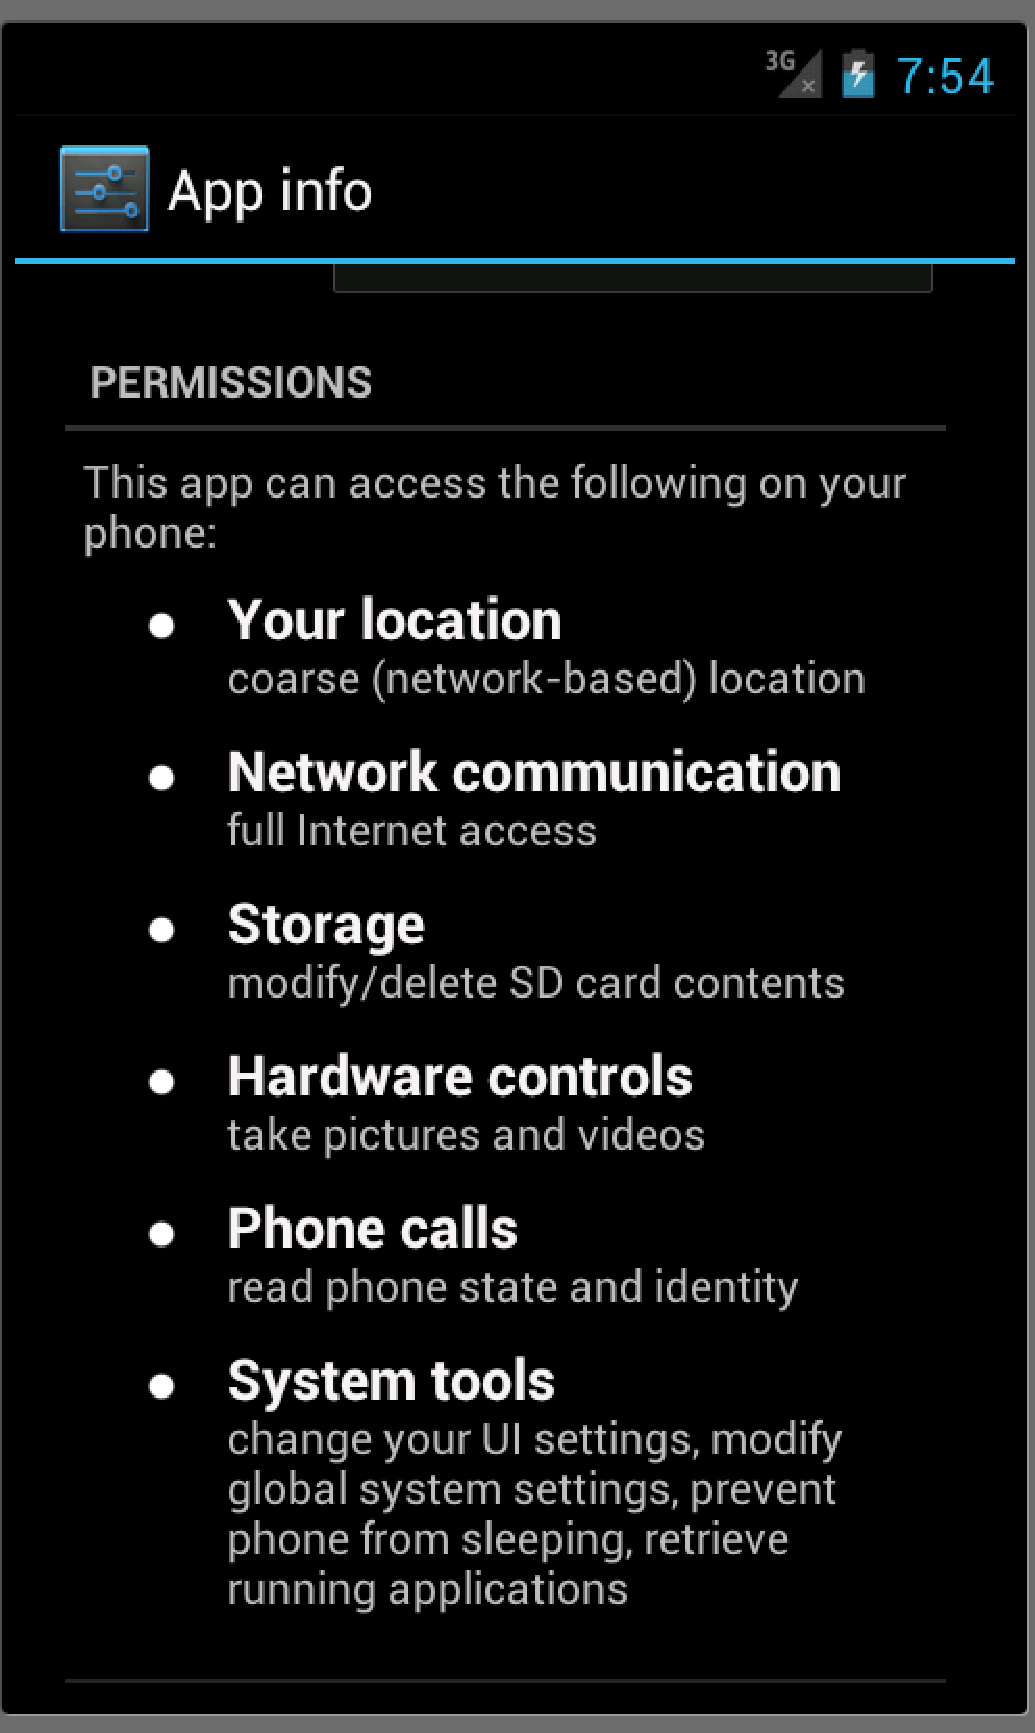
\includegraphics{figure1}}}
\caption{Flashlight app permission requirements}
\label{fig:permission}
\end{figure}

	There are various ways one could remove permissions from Android applications.  Previous work in this area proposes a "privacy mode", where applications running in this mode run with lowered permissions~\cite{Zhou:2011:TISSA}.  This approach requires heavy modification to the Android OS itself, but yields a flexible solution.  Applications can also be repackaged, with their manifests modified to contain fewer permissions.  This is the most popular approach at present, as applications containing this functionality can be readily obtained from major application markets~\cite{Hoffman}.  Additionally, the application's executable code could be dynamically rewritten to protect sensitive API calls~\cite{Davis:2013:RetroSkeleton}.

	All of the above approaches, however, are dependent on Google's policy regarding application permissions, as they influence how developers write their applications. Google's documentation discusses the implementation in enough detail for a developer to use it, but does not go into the rationale behind the approach. While they do suggest that the "dynamic" permission model would be too much of a burden on the user, they do not mention editable static permissions at all. Furthermore, application developers are not explicitly instructed to handle cases of revoked permissions in their applications. Since the lack of a required permission is typically implemented in the form of a Java SecurityException~\cite{Google}, some programmers will handle these gracefully out of habit. However, if an application or library it uses is not explicitly written to handle the permission revocation, modification of the source code will be required to ensure proper function.

\subsection{Effect of Permission Removal}

While previous research has demonstrated that a significant number of Android applications request and use too many permissions~\cite{Felt}, it is unclear how removing permissions would affect the application's behavior.  Under Android's security model, developers typically expect all the requested permissions to be available.  Therefore, it would not be surprising if many developers do not handle the lack of permissions gracefully. When an application invokes an API call without the necessary permissions, it typically throws a \texttt{SecurityException}.  However, if such an exception is caught by library or wrapper code, the application can continue running.  Moreover, permissions are not all equal.  Some permissions describe a devices' hardware capabilities, such as \texttt{CAMERA}.  Since they are not universally available, one would expect libraries to be able to handle their absence more gracefully.  A relatively common instance of this is the removal of the camera on DoD phones for operational security.

When removing a permission, users will expect to see any correlating features be disabled. An everyday example being the removal of GPS capabilities from Google Maps. Currently, many users turn their GPS off in attempts to extend their battery life. When this is done, at launch, the user is notified that the accuracy of Google Maps would be improved if GPS was enabled.  When removing permissions from and application, users are going to expect similar behavior. If an application was not written with permission removal in mind, however, features that are not obviously correlated may malfunction leaving the user confused. This could theoretically include data corruption if the application is not written to handle its data in a robust manner. If this is the case, data would be susceptible to being corrupted if the application crashes regardless of permission removal. While these occurrences are of concern, in the long run, they can easily be addressed by developers.

In this paper, we take the first step to quantitatively measure the effects of removing permissions from Android applications by trying to answer the following questions:

\begin{itemize}
\item How likely will an application crash after a permission is removed?

\item Which permissions, if removed, are less likely to cause an application to crash?

\item Why do applications handle the lack of certain permissions more gracefully?

\end{itemize}

%We chose to test with 7 permissions that we believe have a high potential to result in the compromise of a user's security or privacy.
%While removing a permission may cause many abnormal behaviors, we will focus on crashing, which is likely the most common.  We wish to answer the following questions:
Our work will benefit both users and developers.  Users can make more informed decisions when deciding which permissions to remove (when they use tools for removing permissions).  Application developers can make their code more robust against missing permissions.  Android library developers can design their libraries to handle lack of permissions more gracefully.
	
In the remainder of this paper, we will attempt to quantify the effects of removing permissions from Android applications. In Section \ref{sec:related} we will discuss related work. Then, in Section \ref{sec:method}, we will discuss our methodology and the tool we developed for automated testing, PyAndrazzi. We present the results of our testing in Section \ref{sec:evaluation} and discuss the impact of our findings on users and developers in Section \ref{sec:discussion}. Finally, in Section \ref{sec:future} we discuss future work and conclude with Section \ref{sec:conclusion}. 


% chapter 2
%This is an example for a chapter, additional chapter can be added in the skeleton-thesis
%To generate the final document run latex, build and quick build commands on the skeleton-thesis file not this one.
%This is chapter 2, the default skeleton thesis expects 2 chapters
\chapter{Related Work}
\label{sec:related}
Recently, there have been a number of academic and non-academic works in the area of Android permissions. The work that most closely relates is ~\cite{Hornyack:2011:TAD:2046707.2046780}. In their work, they attempt to analyze the effects of returning fake data to the sensitive API calls who's permissions they want to restrict. The behavioral changes are analyzed by using image comparison techniques. The work performed in this study differs from their's 
in four significant ways. Firstly, the removal of permissions is tested without modifying the Android framework, giving a more realistic  experiment. Secondly, all of the testing is performed autonomously on emulators and does not require human generated application specific scripts, resulting in a scalable testing method. Thirdly,  the samples are used completely random where as their's are significantly skewed towards over permissioned applications which results in an admittedly overestimate of the side effects. Finally, the applications exception behavior is observed instead of using image analysis to detect changes when permissions are removed.  The overall difference is this study attempts to quantify the behavior of an application when a permission is removed, where as ~\cite{Hornyack:2011:TAD:2046707.2046780} focuses on analyzing the effects of using fake instead of removing permissions from applications.   

In ~\cite{Rastogi:2013:AAS:2435349.2435379}, they also performed simlar work.  Like this study, they used UI introspection; however, they utilized humans to record input while the approach utilized in this study generates dynamic input.  In addition, they focus on network traffic while the focus of this research is on an application's on device behavior.  

%A study performed by a team at UC Berkeley found that a large percentage of Android apps were requesting more permissions than they actually used. At the time, Google did not have a complete mapping of Android API calls to the permissions they use; therefore, the team created their own. We made use of this resource often throughout our project~\cite{Felt}. Furthermore, the paper includes a detailed description of the Android permissions mechanism which we will not attempt to duplicate here.

Some third party Android distributions, such as CyanogenMod~\cite{Demers} and MockDroid~\cite{Beresford:2011:MTP:2184489.2184500}, also modify the Android OS to enable permission removal. Like ~\cite{Hornyack:2011:TAD:2046707.2046780}, MockDroid provides fake data to API calls where permissions are being removed. CyanogenMod, however, enables the user to actually revoke permissions. While CyanogenMod essentially accomplishes the changes proposed by this study, the developers of CyanogenMod state concerns about applications failing as a result of permission removal. In addition, these third party distributions are cumbersome to many non-technical users due to the fact that they require you to re-flash the firmware of your device thus voiding its warranty. As a workaround, others have developed applications that allow users to implement the security model described earlier. With the exception of the latest to hit the market, Plop, they all require “rooting”. Among these, LBE Privacy Guard and PDroid provide fake data to handle security exceptions while Plop and Permission Denied do not~\cite{Hoffman}. Using fake data theoretically decreases the number of exceptions incurred, however, it is still unable to handle all of them, i.e. writing to external storage. Ultimately, revoking permissions or providing fake data, regardless of which method one uses, can lead to applications crashing and unexpected behavior. In the end, the better solution is for Google to alter the security model of the Android OS and for developers to handle the exceptions. 


% chapter 3

\chapter{Methodology}
\label{sec:methodology}
%\paragraph{\bfseries Android Over}
%Android is an open source operating system designed for smartphones and other mobile devices whose applications are primarily written in Java, sometimes accompanied by native code, which is then compiled to Dalvik bytecode and run in a virtual machine similar to the Java virtual machine.  Because the quality and trustworthiness of applications varies widely, Android treats all applications as potentially buggy or malicious.  Every application runs as an unpriviledged user with Linux UIDs effectively being used to provide application sandboxes.  To increase code re-usability, the Android application framework forces a componenet-based application model [26].  Instead of having a main() function or any single entry point for execution, Android application of developed in terms of components.

%The applications are composed of four component types:  activity, service, broadcast receiver, and content provider.  Activities are focused windows in which the user interaction takes place; only one activity can be active at a time.  Each activity is a class in the source code and should perform according to events generated by users and the system. Services are designed to run in the background while content providers manage access to data.  Broadcast Receivers are registered with system services and can receive system events, such as re-boot completed, or an SMS received, and so on.  Once a broadcast receiver is registered to receive a system event, the code specified in the broadcast receiver is run whenever the system event is triggered.  Most system events are guarded by permissions, which the applications must declare and get approval for at installation time.

%For automatic exploration, it is neccessary to understand the GUI features in Android.  Each activity corresponds to a screen displayed to the user.  This screen is functionally equivalent to a traditional GUI window, the only difference being that only one screen is shown at a time (with minor exceptions), whereas traditional GUIs can typcally display multiple windows.
%An application's GUI consists of several activities that invoke one another and possibly return results.  At any point in time, only one activity has input focus and processing.  This activity is referred to as the active activity.  When one activity invokes another, the former is paused and the new activity is pushed to the top of the activity stack and made active.  Once an activity has completed its work, it terminates, optionally returning a value, and the next activity on the stack is made active.  Note that activities are not limited to invoking activities within the same application.  A sequence of related activities on the stack is called a task.


%\subsection{Android Overview}   

%Because the quality and trustworthiness of applications varies widely, Android treats all applications as potentially buggy or malicious.  Each application runs in a process with a low-privilege user ID, and applications can access only their own files by default.  Aplications are written in Java (sometimes accompanied by native code), and each application runs in its own Dalvik virtual machine, an optimized Android specific Java VM.  The Android application framework forces a componenet-based application model [26] to increase code reusability.  Applications do not have a main() function or any single entry point for execution but are developed in terms of components.  There are four types of compenents defined in Android's programming model: Activity, Broadcast Receiver, Content Provider and Service. Activity components define an application’s user interface.  Typically, an application developer defines one activity per “screen.” Activities start each other, possibly passing and returning values. Only one activity on the system has keyboard and processing focus at a time; all others are suspended. Service components perform background processing. When an activity needs to perform some operation that must continue after the user interface disappears (such as download a file or play music), it commonly starts a service specifically designed for that action. The developer can also use services as application-specific daemons, possibly starting on boot. Services often define an interface for Remote Procedure Call (RPC) that other system components can use to send commands and retrieve data, as well as register callbacks. Content provider components store and share data using a relational database interface. Each content provider has an associated “authority” describing the content it contains. Other components use the authority name as a handle to perform SQL queries (such as SELECT, INSERT, or DELETE) to read and write content. Although content providers typically store values in database records, data retrieval is implementation-specific—for example, files are also shared through content provider interfaces. Broadcast receiver components act as mailboxes for messages from other applications. Commonly, application code broadcasts messages to an implicit destination. Broadcast receivers thus subscribe to such destinations to receive the messages sent to it. Application code can also address a broadcast receiver explicitly by including the namespace assigned to its containing application.


%Because the quality and trustworthiness of applications varies widely, Android treats all applications as potentially buggy or malicious.  Each application runs in a process with a low-privilege user ID, and applications can access only their own files by default.  Aplications are written in Java (sometimes accompanied by native code), and each application runs in its own Dalvik virtual machine, an optimized Android specific Java VM. The Android operating system limits application privileges through a permission system.  Privileges are requested by the application developer in a manifest which is incorporated into the application package, and approved by the user when the application is installed.  The user may only choose to accept all of the permissions or not install the application -- they can't grant or deny specific permissions.


%Static livraries provide common system and application librariries for applications.  The Android runtime environment is composed of core runtime libraries and the Dalvik virtual machine (VM) - an optimized Android-sepcific Java virtual machine.  Finally the Linux kernel completes the OS and the software stack.  Each Android application runs with a unique user ID, in its own copy of the Dalvik virtual machine, which ensures separation between applications and provides protection.
 
%Android controls access to system resources with installtime permissions categorized into three threat levels : Normal, Dangerous, and Signature/System.  Applications can define their own permissions for purpose of self-protection.  Permissions may be required when interacting with the system API, databases, and the message-passing system.

%This work involves the top three layers.  To test programs running in the Application layer, services from the Application Framework layer and intrumentation tools in the Dalvik VM are used.

%Andorid applications can be composed of four component categores: Activity, Broadcast Receiver, Content Provider and Service.  
%Android defines four component
%types:





%The activity GUI layout is commonly defined in XML but may also be defined programmatically.  As in traditional GUIs, an Android window consists of widgets, which are referred to as views in Android terminology.  The Android library supplies several useful views which may either be standalone (e.g., buttons) or act as containers for other views.  In addition to the window layout, an activity can define a menu that appears when the user presses the physical "Menu" button on the phone.

%Applications run at the very top of the platform with their Services, such as the Acitivity Manager , which controls the activities for each application and Content Providers, which load the content provider defined by each application while restricting data accessibility across applications, located in the Application Framework layer


\toolname, a system for evaluating how removing permissions impacts the behavior of Android applications, was designed for the purpose of this study and leverages the Android emulator, APKTool, and AndroidViewClient.  To evaluate each application, \toolname\ automatically runs the application, supplies it with various UI events, detects when the application crashes, and logs the cause of the crash.  \toolname\ consists of the following components (see Figure~\ref{fig:diagram}).

%\FloatBarrier
\begin{figure*}[b]
\figsp
\centerline{\resizebox{0.9\linewidth}{!}{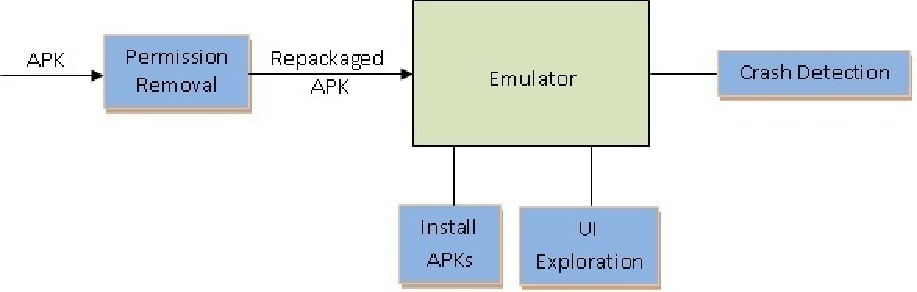
\includegraphics{flowchart}}}
\caption{PyAndrazzi Component Diagram}
\label{fig:diagram}
\end{figure*}
%\FloatBarrier

%\FloatBarrier
\begin{figure*}[b]
\centerline{\resizebox{0.5\linewidth}{!}{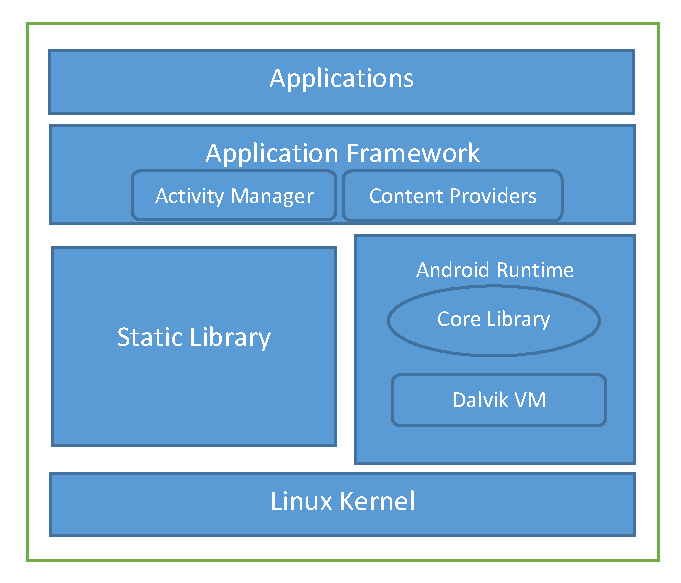
\includegraphics{android_architecture}}}
\caption{Android Platform Architecture}
\label{fig:architecture}
\end{figure*}
%\FloatBarrier

\paragraph{\bfseries Android Emulator}
The Android platform is comprised of 4 layers: Applications, an Application Framework layer, a Library/VM layer, and, the Linux Kernel (see Figure \ref{fig:architecture}).  Applications run at the very top of the platform with their Services, such as the Acitivity Manager and Content Providers, located in the Application Framework layer.  The Library/VM layer contains static libraries and the Android runtime environment.  An Android emulator is an application that provides a virtual mobile device on which Android applications can be run.  It runs a full Android system stack, down to the kernel level, that includes a set of pre-installed applications, such as the dialer, that applications can access.  The emulator provides dynamic binary translation of device machine code to the OS and processor architecture of the development machine.  The configuration of AVDs(Android Virtual Devices), allows for the specification of the Android platform (i.e. API 17) to run in the emulator, the set of hardware options and the emulator skin.  The Android system images, available through the Android SDK Manager, contain code for the Android Linux kernel, the native libraries, the Dalvik VM, and the various Android packages (such as the Android framework and pre-installed applications).  



The Android SDK Manager provides system images for both x86 and arm architectures, however, the x86 image does not include the map libraries.  To improve performance, \toolname~employs the x86 architecture and kvm acceleration, and utilizes a modified x86 system image that includes the missing libraries.  When launching an emulator, the desired AVD configuration is specified.  Each AVD functions as an independent device, with its own private storage for user data, SD card, etc. 

%When launchincg the emulator with an AVD configuration, it automatically loads the user data and SD card data from the AVD directory. By default, the emulator stores the user data, SD card data, and cache in the AVD directory.

\subsection{Android Applications}
Because the quality and trustworthiness of applications varies widely, Android treats all applications as potentially buggy or malicious.  Every application runs as an unprivileged user with Linux UIDs effectively being used to provide application sandboxes; by default, applications are only permitted to access their own files.  To increase code re-usability, the Android application framework forces a component-based application model~\cite{4768655}.  Instead of having a main() function or any single entry point for execution, Android applications are developed in terms of components.  The applications are composed of four component types:  activity, service, broadcast receiver, and content provider.  Activities are focused windows in which the user interaction takes place; only one activity can be active at a time.  Each activity is a class in the source code and should perform according to events generated by the user and system.  Services are designed to run in the background while content providers manage access to data.  Broadcast Receivers are registered with system services and can receive system events, such as re-boot completed, or an SMS received, etc.  Most system events are guarded by permissions, which the applications must declare and get approval for at installation time.  As previously discussed, all permissions are requested by the application developer in a manifest which is incorporated into the application package and approved by the user at install-time.  

%In the current implementation, application developers are responsible for defining the set of permissions their application “requires” independent of what their application’s code actually uses~\cite{Felt}.  The list is presented to the user at install-time whether installing an application obtained through the Google Play market or elsewhere.  This list contains the canonical names given to each permission object, but provides little context as to what the permission is being utilized for.  At the end of the day, however, users have no choice but to accept all of the permissions or not install the application; they can't grant or deny specific permissions.

\paragraph{\bfseries Permission Removal}
APKTool is an opensource tool developed for reverse engineering closed, binary Android applications. It decompiles bytecode to smali, an assembly language for the dex format used by Android's Davlik VM, and is able to re-build applications after modifications are made.  \toolname\ uses APKTool to decode the application's APK file.  Then, it removes the permission being evaluated from the applications AndroidManifest.xml file and collects the Activity names for use in automated testing.  Finally, it rebuilds the APK and signs it using Android's built-in debug key.



\paragraph{\bfseries Installation and Execution}
\toolname\ installs and runs applications in emulators.  It utilizes the standard android debug bridge(ADB) to install and uninstall applications and, due to its increased stability, uses the android debug bridge(ADB) developed by ~\cite{Milano} to provide UI inputs to applications.

%For automatic exploration, it is neccessary to understand the GUI features in Android.  Each activity corresponds to a screen displayed to the user.  This screen is functionally equivalent to a traditional GUI window, the only difference being that only one screen is shown at a time (with minor exceptions), whereas traditional GUIs can typcally display multiple windows.
%An application's GUI consists of several activities that invoke one another and possibly return results.  At any point in time, only one activity has input focus and processing.  This activity is referred to as the active activity.  When one activity invokes another, the former is paused and the new activity is pushed to the top of the activity stack and made active.  Once an activity has completed its work, it terminates, optionally returning a value, and the next activity on the stack is made active.  Note that activities are not limited to invoking activities within the same application.

\paragraph{\bfseries Automatic UI Exploration}
The approach utilized in this study does not attempt to replicate how a user would exercise and application.  \toolname\ needs to execute as much code as possible to maximize the number of adverse effects resulting from permission removal.  Thus, to maximize coverage, \toolname\ takes the list of Activities for each application and executes each one starting with the \texttt{Main} Activity.  During each Activity, \toolname\ performs a series of pseudo-random screen touches.  This functionality is implemented using a UI introspection approach based on the AndroidViewClient library~\cite{Milano}.  Using this method, \toolname\ is able to query the screen for click-able elements and perform "random" touches with a high probability of changing the application state.  Since not all activities are meant to be executed by the user, many are supposed to be called by another activity, this approach will result in a high number of exceptions.  Since the focus of this study is to trigger \texttt{SecurityExceptions}, the resulting high number of exceptions is acceptable since the completion of a baseline evaluation enables the exceptions resulting from permission removal to be identified.      

\paragraph{\bfseries Crash Detection}
Because only one activity has input focus and processing a any point in time, \toolname\ is able to communicate with the emulator's ActivityManager monitor to watch for and acquire data on all crash events and their associated package and activity names.  When an application crashes due to a fatal error, such as a \texttt{SecurityException}, a separate thread communicating with the emulator's ActivityManager, notifies the testing thread, which records the cause of the crash and launches the next Activity.  A similar sequence occurs when a touch results in leaving an application (i.e. opening the browser); the thread communicating with Android's ActivityManager, detects that the application is no longer running in the foreground and notifies the testing thread, which then touches the back button.  This ensures the exceptions generated are from the specific application in question.


% chapter 4
%This is an example for a chapter, additional chapter can be added in the skeleton-thesis
%To generate the final document run latex, build and quick build commands on the skeleton-thesis file not this one.
%This is chapter 2, the default skeleton thesis expects 2 chapters
\chapter{Results}
\label{sec:evaluation}

To evaluate the impact of removing permissions on applications, seven common permissions (Table~\ref{tbl:results}) were selected based on their potential threat to the user's security and privacy.  For each permission, 100 applications that declare the permission in their manifests were randomly downloaded.  These applications are from the official Google Play Market as well as other markets in the US, China, and Europe.

\begin{table*}[t]
\centering
\tiny
\begin{tabular}{|l|c|c|c|c|}
\hline
& \# Failed & \# Apps & \multicolumn{2}{|c|}{\texttt{SecurityException}} \\ \cline{4-5}
Data Set & APKTool & Run & \# Exceptions & \# Apps Throwing Exceptions\\ \hline 
{\bfseries \ttfamily WRITE\_SMS} Original & 0 & 99 & 0 & 0 \\ \hline
{\bfseries \ttfamily WRITE\_SMS} Removed & 0 & 99 & 0 & 0 \\ \hline
{\bfseries \ttfamily ACCESS\_FINE\_LOCATION} Original & 0 & 100 & 2 & 2 \\ \hline
{\bfseries \ttfamily ACCESS\_FINE\_LOCATION} Removed & 1 & 99 & 21 & 12 \\ \hline					
{\bfseries \ttfamily CAMERA} Original & 1 & 99 & 0 & 0 \\ \hline
{\bfseries \ttfamily CAMERA} Removed & 2 & 98 & 0 & 0 \\ \hline
{\bfseries \ttfamily RECORD\_AUDIO} Original & 0 & 100 & 0 & 0 \\ \hline
{\bfseries \ttfamily RECORD\_AUDIO} Removed & 4 & 96 & 0 & 0 \\ \hline
{\bfseries \ttfamily READ\_CALENDAR} Original & 0 & 99 & 0 & 0 \\ \hline 
{\bfseries \ttfamily READ\_CALENDAR} Removed & 0 & 99 & 19 & 6 \\ \hline
{\bfseries \ttfamily READ\_CONTACTS} Original & 1 & 99 & 0 & 0 \\ \hline
{\bfseries \ttfamily READ\_CONTACTS} Removed & 3 & 97 & 81 & 18 \\ \hline
{\bfseries \ttfamily INTERNET} Original & 0 & 99 & 84 & 3 \\ \hline
{\bfseries \ttfamily INTERNET} Removed & 0 & 99 & 84 & 3 \\ \hline
\end{tabular}
\caption{Results of Random UI Introspection}
\label{tbl:results}
\end{table*}


A small portion (less than 2\%) of the applications contained manifests with unusual control characters that APKTool would not process (eg. 0x04), and were discarded.  Additionally, acouple of the applications failed installation and consequently were not tested. \toolname\ installed and tested the remaining ones as described in Chapter~\ref{sec:methodology}. 

\toolname\ detects application crashes and their causes from the emulator's ActivityManager.  When an application does not have a permission required by an API call, the Android framework will typically throw a \texttt{SecurityException} and, unless it catches the exception, the application will crash.   For example, this occurs if there are bugs in the application, or when \toolname\ executes an activity that is not meant to be executed by the user.  An additional possibility is that a library acting on the application's behalf receives the \texttt{SecurityException} and returns the improper error condition.  Applications that do not check for this kind of error state may crash with other types of exceptions such as \texttt{NullPointerException}.  To get an idea of what new errors, besides \texttt{SecurityExceptions}, might be thrown when a permission is removed, all the exceptions are tracked and plotted as you will see below.  Ultimately, since it is not possible to determine the true causes of these exceptions without extensive static analysis of each application, this study focuses on \texttt{SecurityExceptions}, which indicate under-permission.  The seven permissions and their application crash patterns are examined separately below.

%Among all the crashes, 5.8\% were due to a \texttt{SecurityException}.

\paragraph{\bfseries \ttfamily INTERNET}
From a thorough examination of the logs, it was ascertained that the \texttt{SecurityExceptions} generated both before and after permission removal were the result of a change in the permissions system in Android 4.2.  For the API calls the applications performed, Android 4.2 requires a new permission, \texttt{WRITE\_APN\_SETTINGS}.  This is technically under-permission, but was not caused by removing existing permissions.  For the remainder of the sample set, ad libraries were the sole reason for an application's request for the \texttt{INTERNET} permission.  All the versions of the \textit{AdMob} libraries that were examined fail gracefully when the INTERNET permission was removed.  For example,  one version of \textit{AdMob} displays a message to the user as seen in Figure~\ref{fig:removing}. 
%\FloatBarrier
\begin{figure}[h!]
\centerline{\resizebox{0.3\linewidth}{!}{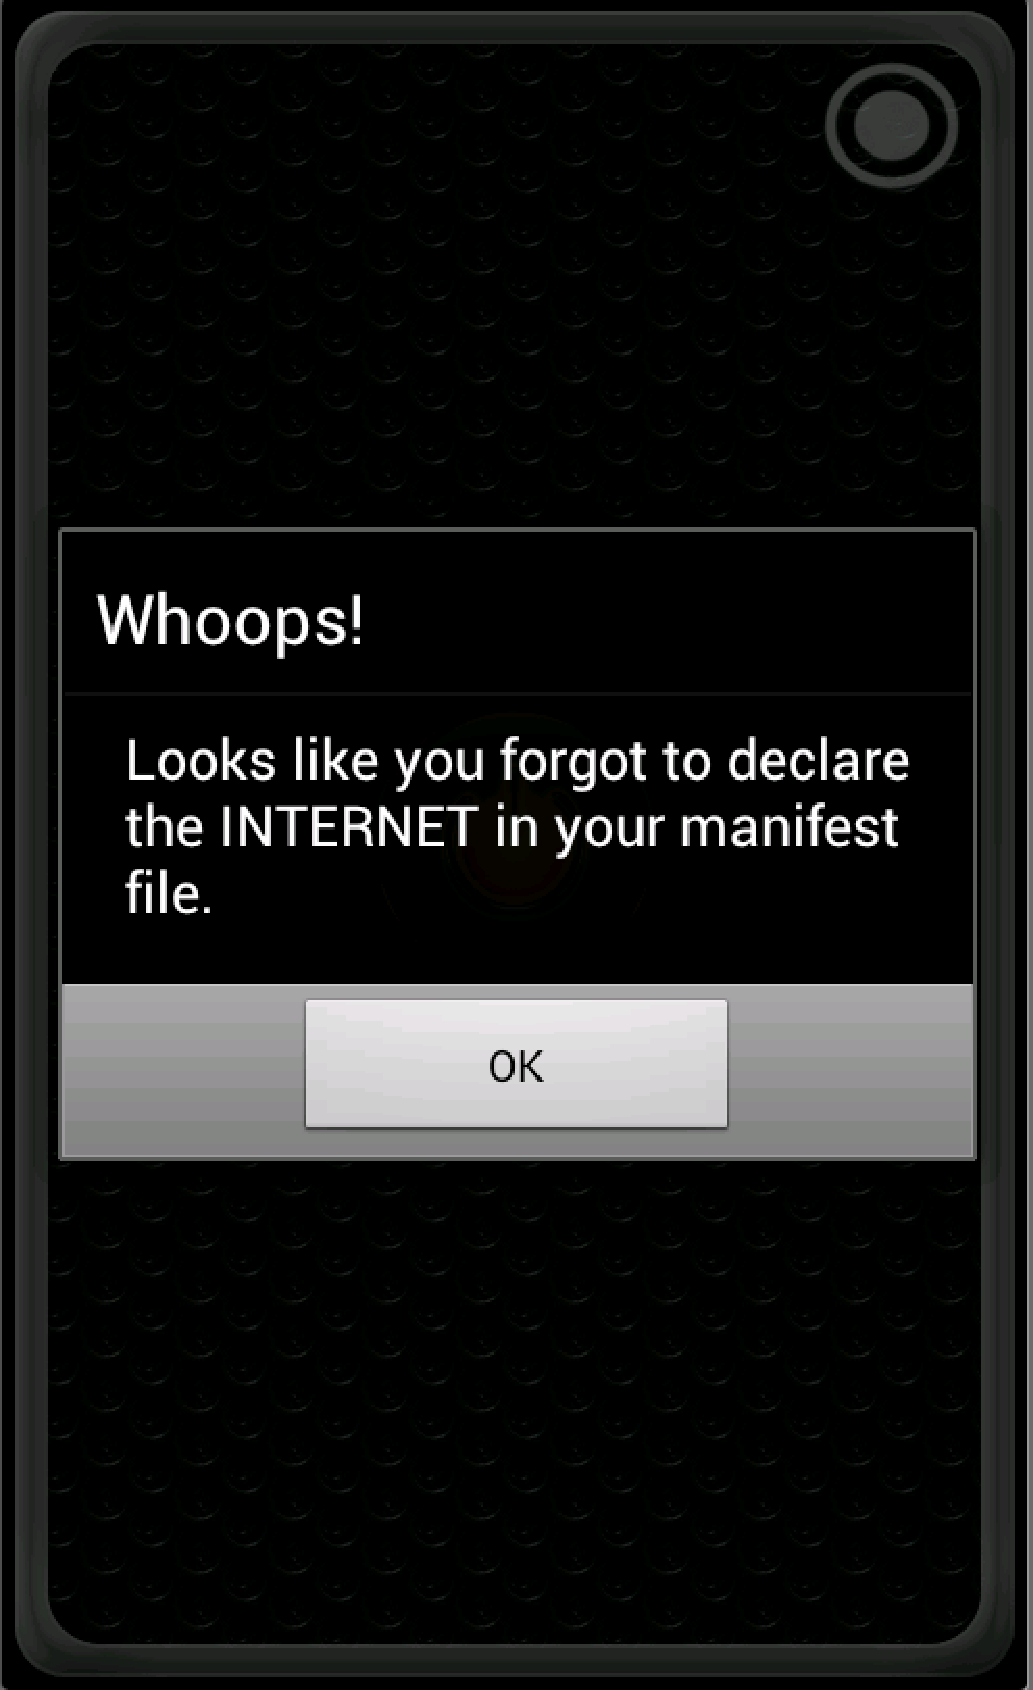
\includegraphics{figure2}}}
\caption{Admob displays a message when the \texttt{INTERNET} permission is removed.}
\label{fig:removing}
\end{figure}
%\FloatBarrier
In light of this, a copy of a popular third-party Android web browser was attained and its \texttt{INTERNET} permission removed using \toolname. When executed, the application terminated with a \texttt{SecurityException} related the applications request for DNS information. With further investigation it was determined that the application calls the \texttt{java.net} functions directly, causing a \texttt{SecurityException} to be generated and the standard crash screen to be displayed (see Figure~\ref{fig:crash}).


%\FloatBarrier
\begin{figure}[h!]
\hfill
\subfigure[]{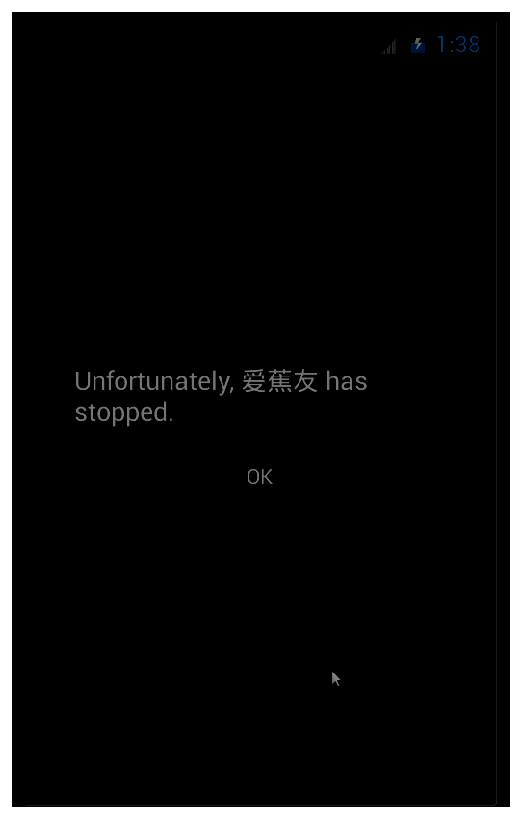
\includegraphics[scale=0.7]{figure3}\label{fig:crash}}
\hfill
\subfigure[]{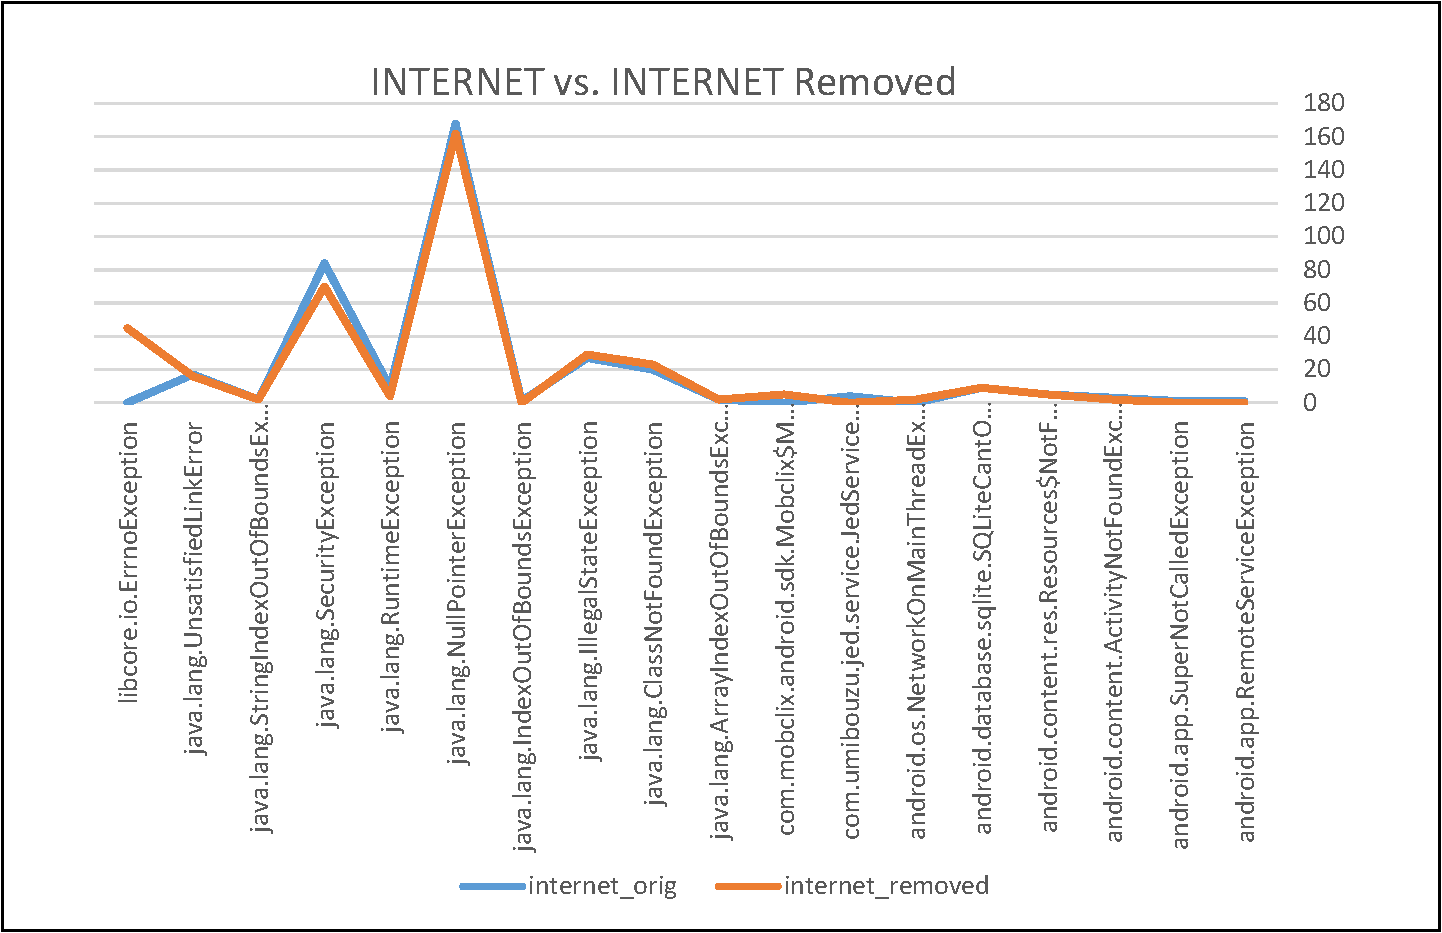
\includegraphics[width=8cm]{internet}\label{fig:internet}}
\hfill
\caption{App crashes due to \texttt{SecurityException} when the \texttt{INTERNET} permission is removed~\ref{fig:crash} and Distribution of Exceptions with \texttt{INTERNET} permission~\ref{fig:internet}.}
\end{figure}
%\FloatBarrier
When alanyzing the exception patterns of testing the applications with and without the \texttt{INTERNET} permission, there was no significant change in the exception behavior (Figure~\ref{fig:internet}). 

%\begin{figure}[t]
%\centerline{\resizebox{0.8\linewidth}{!}{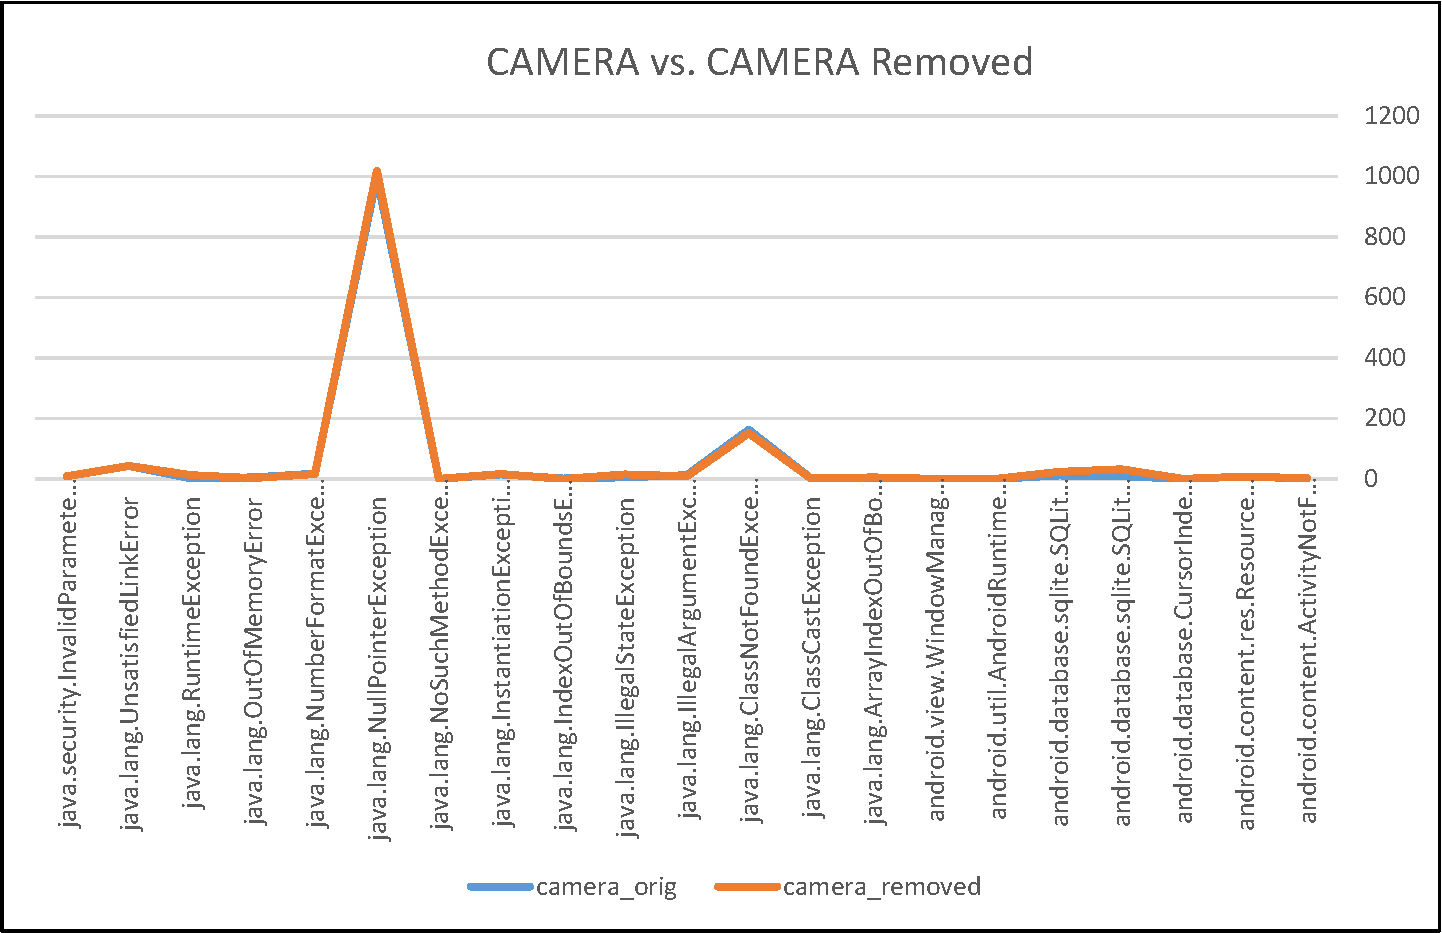
\includegraphics{camera}}}
%\caption{Distributiont of Exceptions for \texttt{CAMERA} permission.}
%\label{fig:camera}
%\end{figure}

%\begin{figure}[t]
%\centerline{\resizebox{0.8\linewidth}{!}{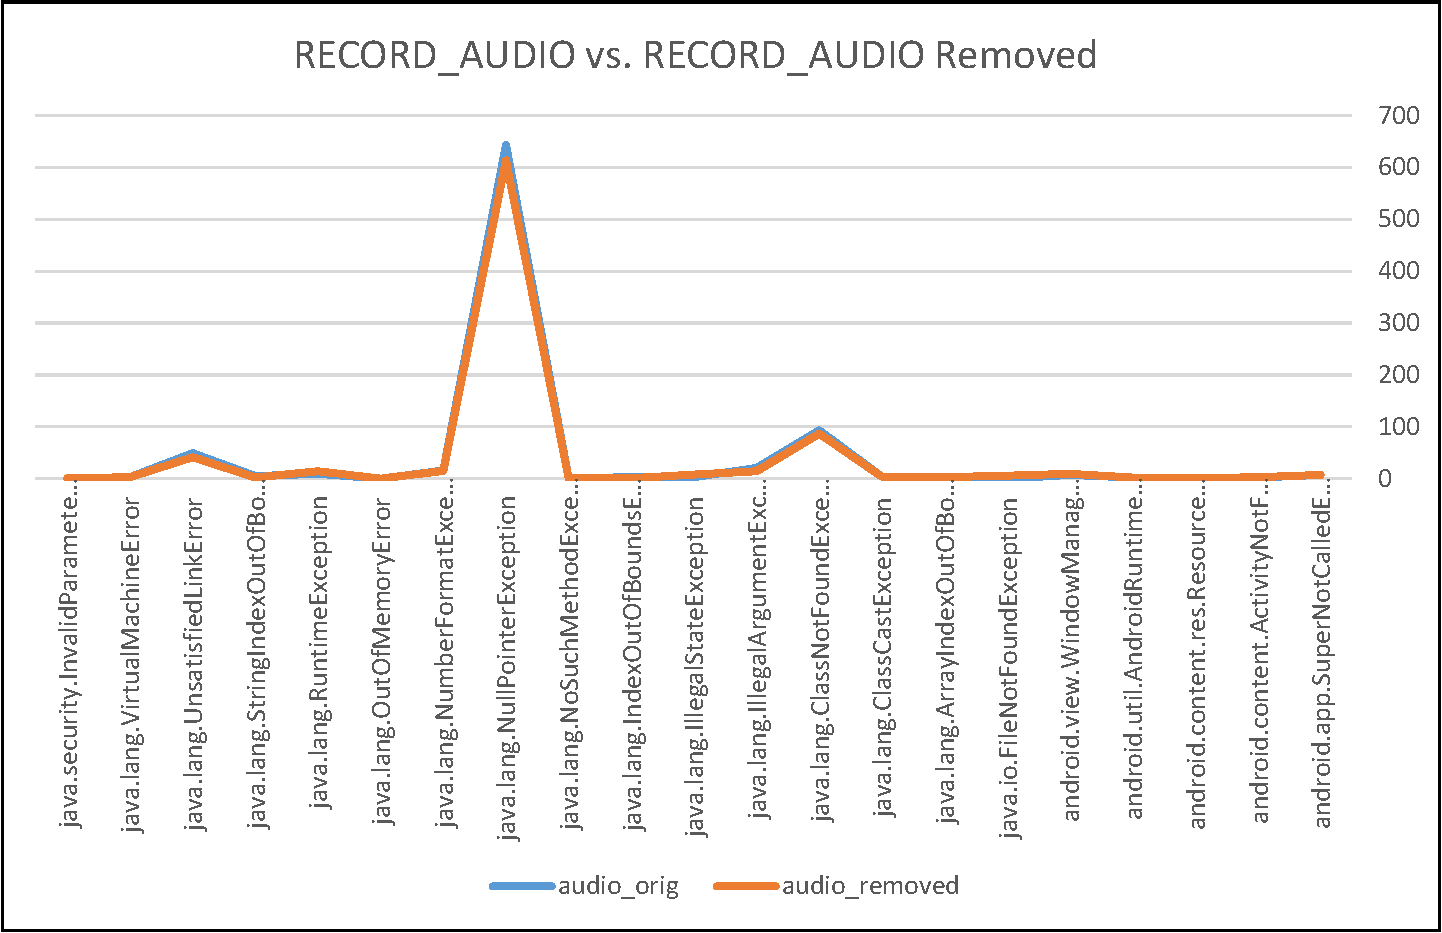
\includegraphics{audio}}}
%\caption{Distributiont of Exceptions for \texttt{RECORD\_AUDIO} permission.}
%\label{fig:audio}
%\end{figure}

\paragraph{{\bfseries \ttfamily CAMERA} and {\bfseries \ttfamily RECORD\_AUDIO}}
In the case of \texttt{CAMERA} and \texttt{RECORD\_AUDIO}, both functionalities have a service that proxies application requests.  If the relevant permissions are removed, they will behave as if no camera or microphone is present.  Therefore, no \texttt{SecurityExceptions} were observed when these permissions were removed and the exception behavior of the applications showed no significant change (see Figure~\ref{fig:camera} and~\ref{fig:audio}).
%\FloatBarrier
\begin{figure}[h!]
\hfill
\subfigure[]{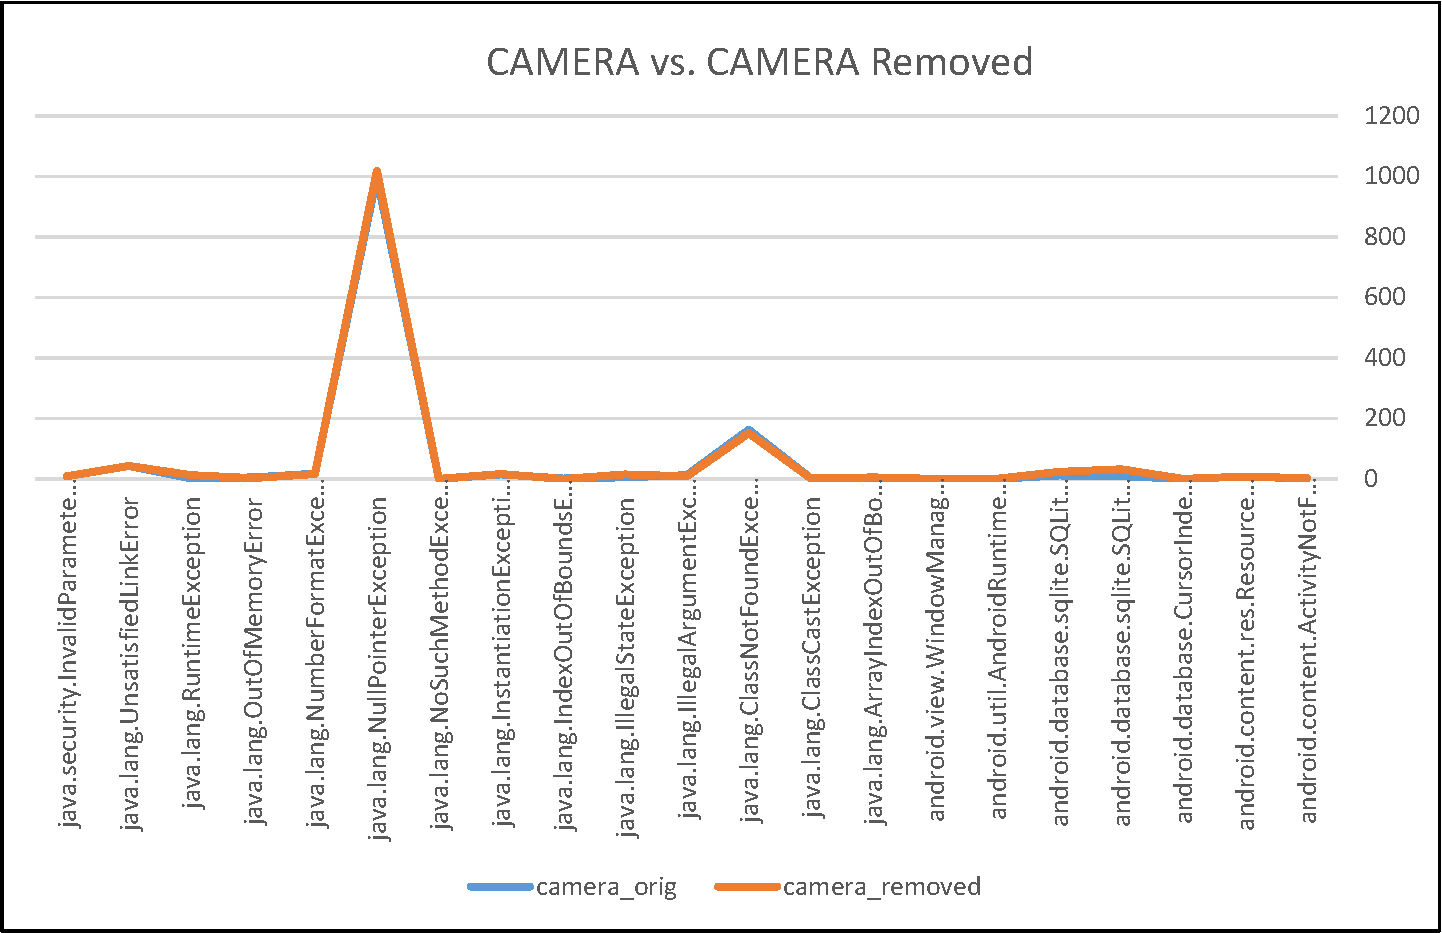
\includegraphics[width=8cm]{camera}\label{fig:camera}}
\hfill
\subfigure[]{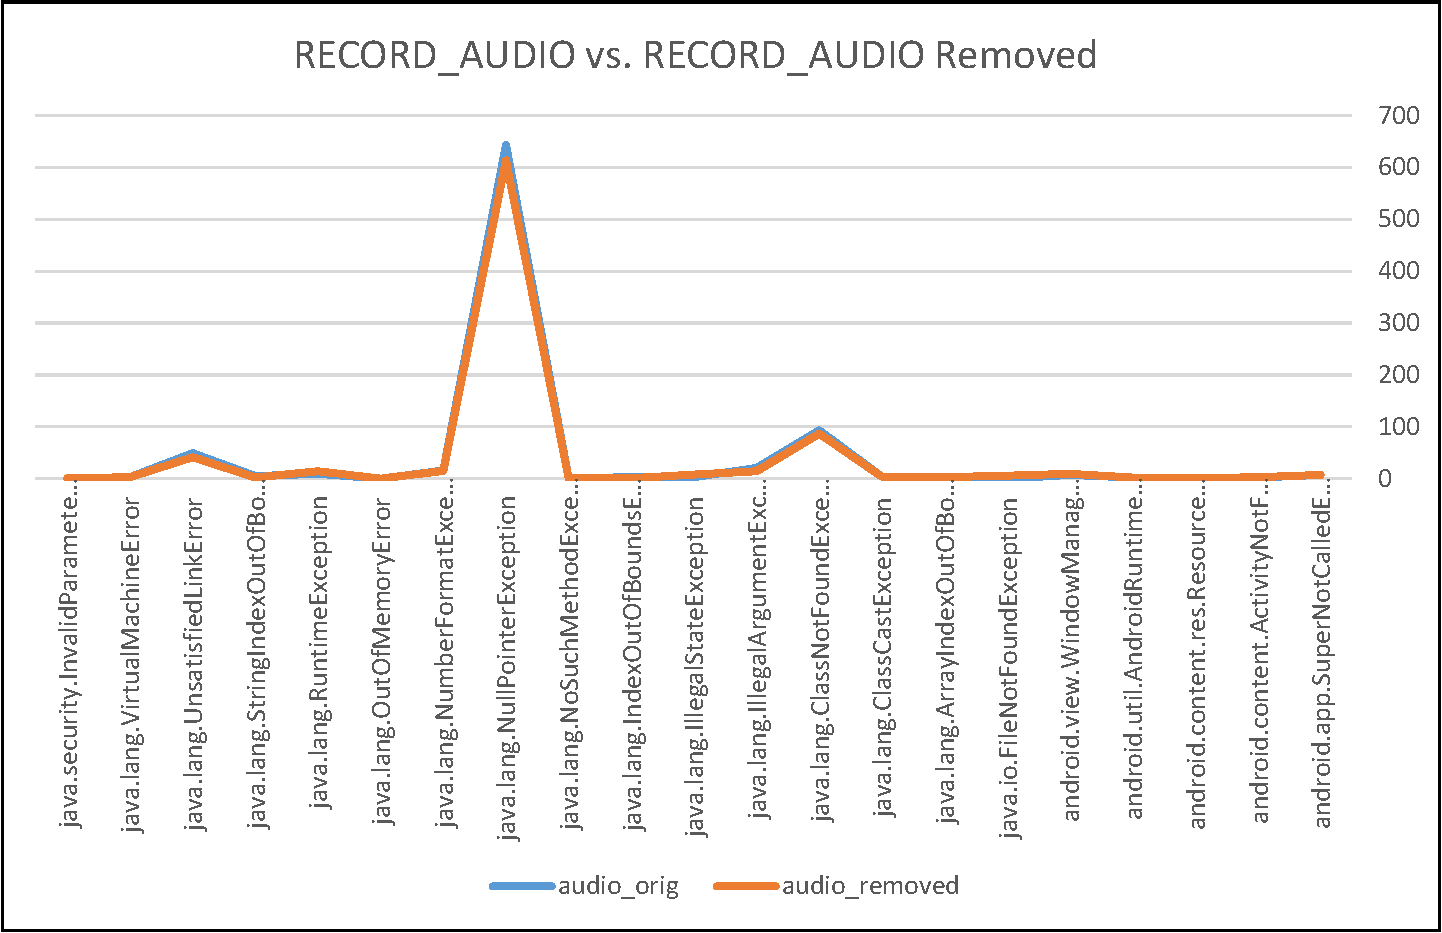
\includegraphics[width=8cm]{audio}\label{fig:audio}}
\hfill
\caption{Distribution of Exceptions for \texttt{CAMERA}~\ref{fig:camera} and \texttt{RECORD\_AUDIO}~\ref{fig:audio} permissions}
\end{figure}
%\FloatBarrier

\paragraph{{\bfseries \ttfamily READ\_CONTACTS} and {\bfseries \ttfamily READ\_CALENDAR}}
Manual investigation determined that, when removing \texttt{READ\_CONTACTS}, a \texttt{SecurityException} was only being recieved in cases where the API call to read the contacts was actually occurring. While the presence of some other helper library that catches exceptions cannot be completely ruled out, in every case that was manually examined, the \texttt{SecurityException} was only occurring when the automated testing specifically activated a UI element or activity's startup code that made a request to the Provider URI, \texttt{content://com.android.contacts/}. 

The removal of \texttt{READ\_CALENDAR} results in similar behavior. Apps attempting to access the Provider URI, \texttt{content://com.android.calendar/}, generated security exceptions in all cases that were examined.  When looking at the exception distribution plots for \texttt{READ\_CALENDAR} and \texttt{READ\_CONTACTS}, both show the expected difference when their respective permissions are removed.  In the case of \texttt{READ\_CONTACTS}, however, there is an additional difference due to \texttt{com.scoreloop.client.android.ui.StandardScoreloopManager\$VerifyException}.  This error is due to an applications use of ScoreLoop, a cross-platform gaming SDK.  The SDK requires the \texttt{READ\_CONTACTS} permission and has its own exception handler written for when it is not declared in the manifest.

%\FloatBarrier
\begin{figure}[h!]
\hfill
\subfigure[]{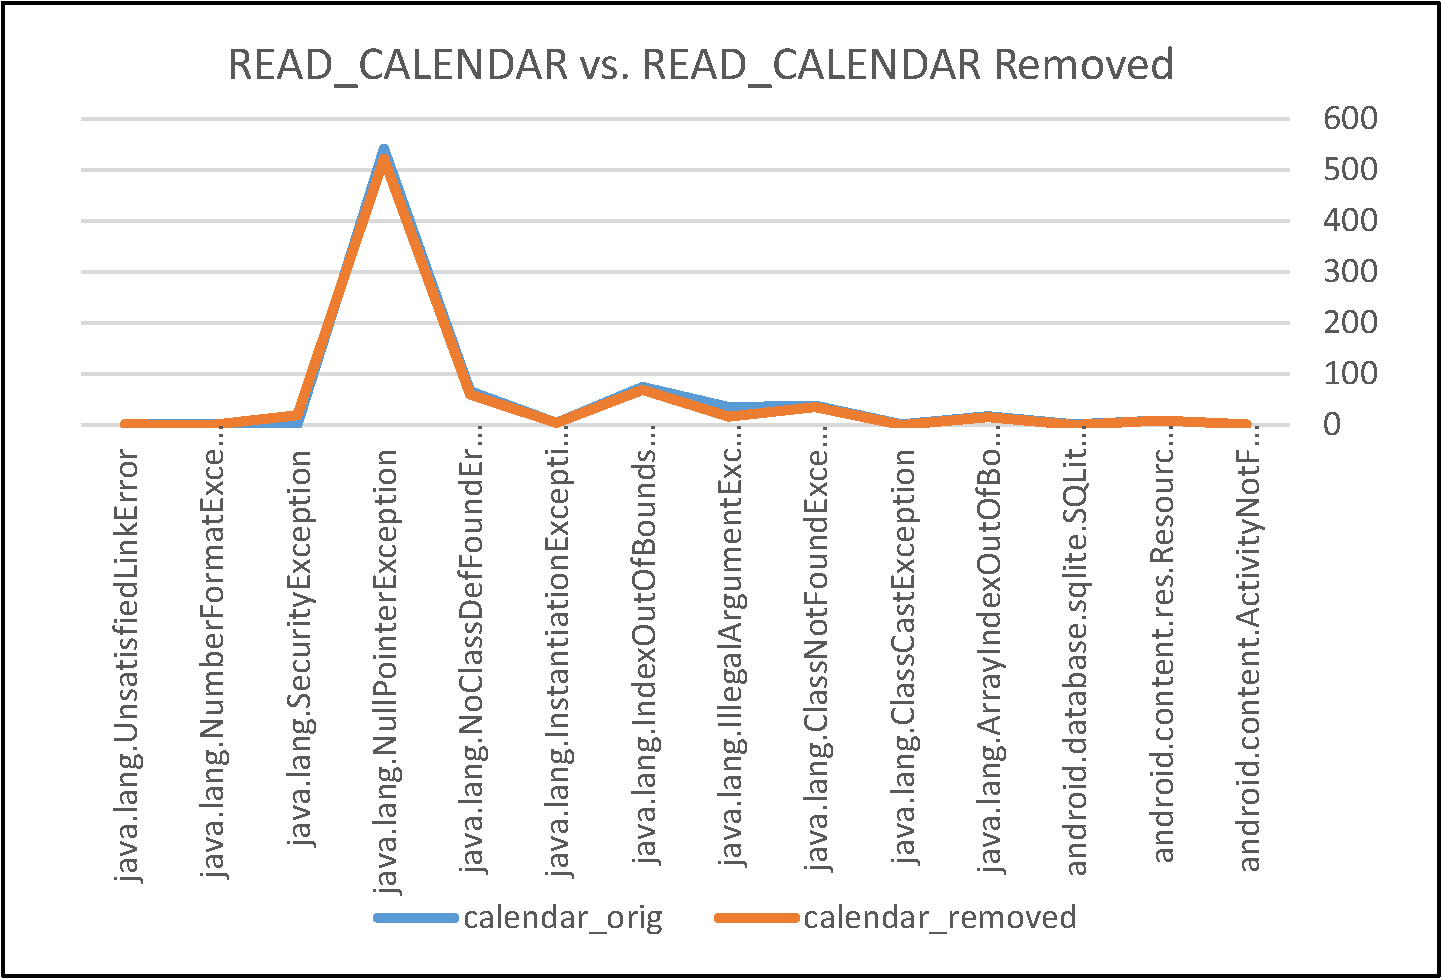
\includegraphics[width=8cm]{calendar}\label{fig:calendar}}
\hfill
\subfigure[]{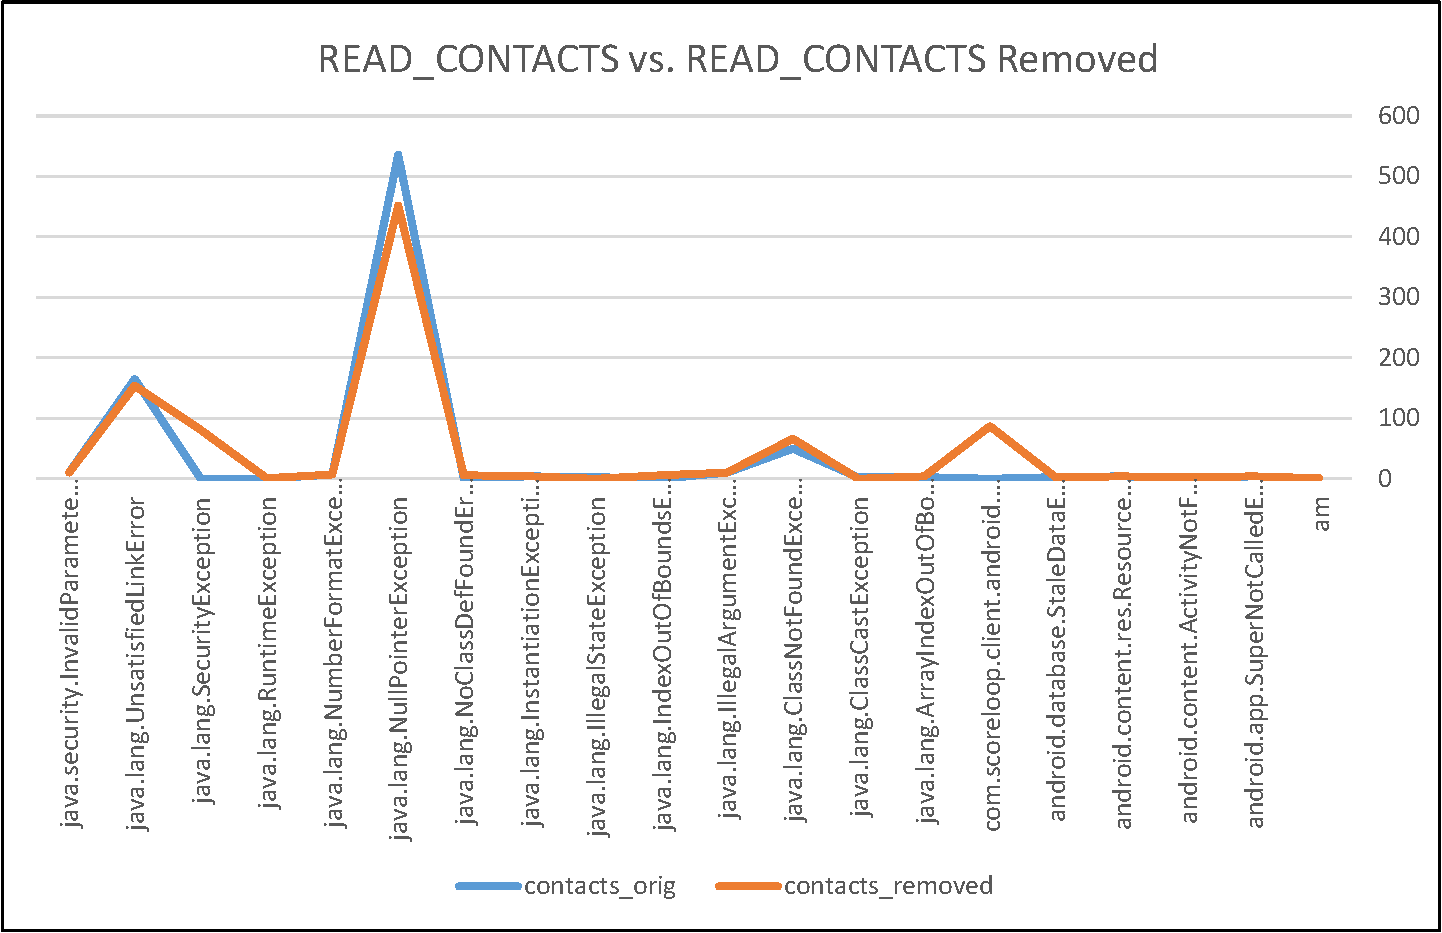
\includegraphics[width=8cm]{contacts}\label{fig:contacts}}
\hfill
\caption{Distribution of Exceptions for \texttt{READ\_CALENDAR}~\ref{fig:calendar} and \texttt{READ\_CONTACTS}~\ref{fig:contacts} permissions}
\end{figure}
%\FloatBarrier

\paragraph{\bfseries \ttfamily WRITE\_SMS}
The \texttt{WRITE\_SMS} permission also uses a Provider URI, \texttt{content://mms-sms/}; however, no \texttt{SecurityExceptions} resulting from permission removal were observed.  The one that was observed in both test cases was a result of the missing permission, \texttt{WRITE\_APN\_SETTINGS}, that was discussed earlier.  The lack of \texttt{SecurityExceptions} is likely due to the relative depth of writes to this URI within the application, which makes it more difficult to trigger.  Any unauthorized Provider URI access produces the standard crash screen (Figure~\ref{fig:crash}).  As expected, with no \texttt{SecurityExceptions} triggered, there was not significant difference in the distribution of errors with or without the permission. 

%\FloatBarrier
\begin{figure}[h!]
\hfill
%\subfigure[\texttt{WRITE\_SMS} permission]{\includegraphics[width=8cm]{sms-crop}}
\subfigure[]{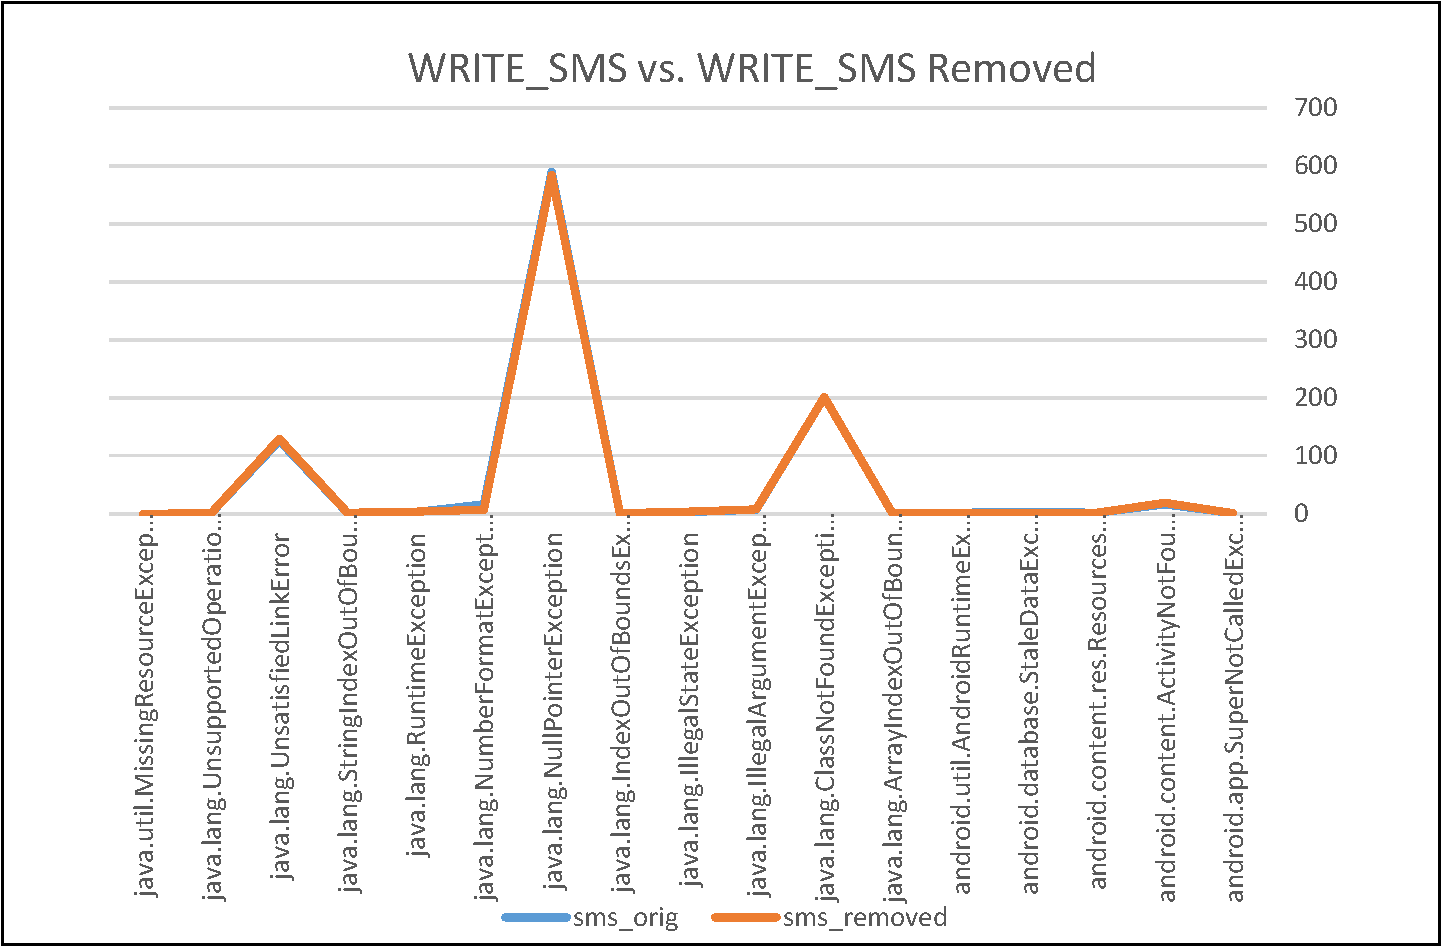
\includegraphics[width=8cm]{sms}\label{fig:sms}}
\hfill
%\subfigure[\texttt{ACCESS\_FINE\_LOCATION} permission]{\includegraphics[width=8cm]{location-crop}}
\subfigure[]{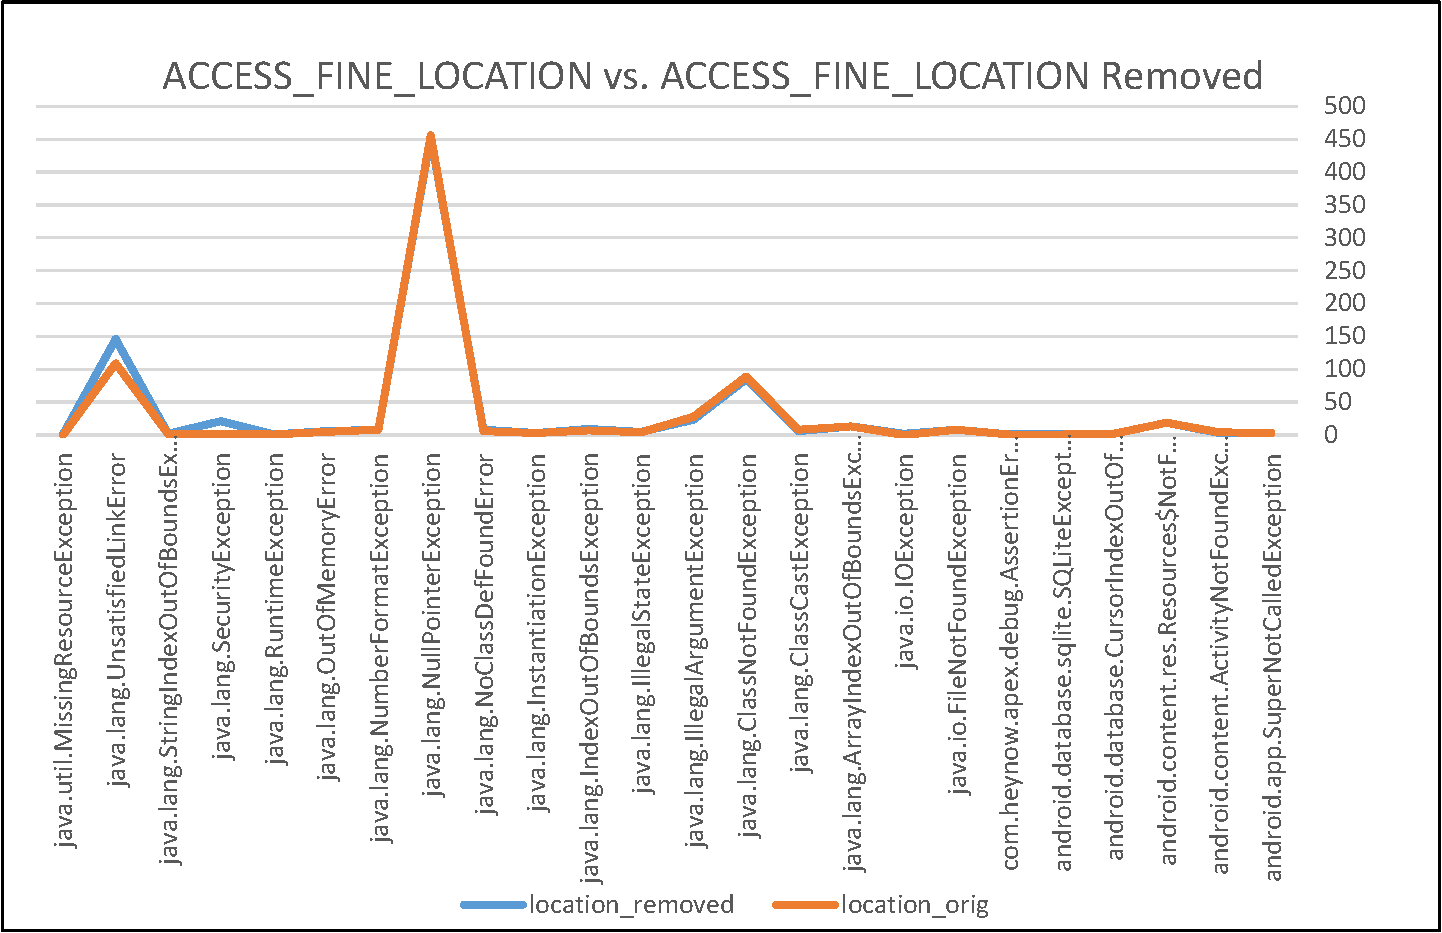
\includegraphics[width=8cm]{location}\label{fig:location}}
\hfill
\caption{Distribution of Exceptions for \texttt{WRITE\_SMS}~\ref{fig:sms} and \texttt{ACCESS\_FINE\_LOCATION}~\ref{fig:location} permissions.}
\end{figure}
%\FloatBarrier

\paragraph{\bfseries \ttfamily ACCESS\_FINE\_LOCATION}
The fine-grained location permission, \texttt{ACCESS\_FINE\_LOCATION}, is a special case. It is one of a few permissions in Android that is a nested permission. Many API calls will operate in the presence of either fine or coarse location permissions but prefer fine; if fine is removed they will fall back to coarse grain location. This results in few \texttt{SecurityExceptions} (\textasciitilde12\%), since they will only occur in cases where the GPS hardware is explicitly being used.  Comparing the distribution of exceptions, the removal of the \texttt{ACCESS\_FINE\_LOCATION} permission does not appear to have any significant impact on exceptions outside of causing \texttt{SecurityExceptions}.


% chapter 5

\chapter{Discussion}
\label{sec:discussion}

The evaluation shows that the rate of failure varies with the permission.  In this test, removing permissions only caused 38 (5.3\%) of the 685 applications to crash due to a type of \texttt{SecurityException}.   In the best cases, removing \texttt{CAMERA}, \texttt{RECORD\_AUDIO} and \texttt{WRITE\_SMS} respectively, never caused crashes due to permission removal.  While the random sample did not result in any \texttt{SecurityExceptions} with the removal of \texttt{WRITE\_SMS}, it is probable that this is due to the API call being triggered by UI elements deep in the UI structure.  Furthermore, the results from the random sample showed that, if an application's sole use of the \texttt{INTERNET} permission is for advertising, \texttt{SecurityExceptions} caused by its removal are likely to be handled by the ad library.  If the application makes use of network functionality on its own, as in the manually selected test case, the application may crash with a \texttt{SecurityException}. Lastly, it was determined that removing the \texttt{READ\_CONTACTS} and \texttt{ACCESS\_FINE\_LOCATION} permissions had the greatest impact causing 19 and 12 applications to crash respectively.      

\paragraph{\bfseries Wrapper Code}
The manual inspection shows that many wrapper code pieces handle the lack of permissions gracefully.  Wrapper code includes both system services such as Audio Manager and Camera, as well as developer-defined libraries like those used for advertising and the ScoreLoop SDK.  System services provide abstraction between \texttt{getHostByName()} in the developer's code and the hardware.  For example, an application trying to use the device's camera can fail gracefully in the event the device has no camera.  This is also true of permissions revocation.  When the relevant permission is removed, the service acts as if the hardware it manages does not exist.  Third-party libraries can accomplish the same feat by catching the exception on behalf of the developer.  Google AdMob, for example, will display a message to the user running an application without the necessary permissions to obtain the ads (See \ref{fig:removing}).  Notably, it will allow the application to continue to function without advertising.  

While these wrapper code pieces make it easier for the user to remove the permission without causing crashes, they make it harder for the developer to detect the lack of declared permissions programmaticaly.  To address this, developers could make their own API calls to force the exception to be thrown if they wanted to take their own action on permissions revocation as is done by the Scoreloop SDK. 

\paragraph{\bfseries Protected URI}
In situations where an application accesses protected URIs directly (not through wrapper code), it was verified that the application throws \texttt{SecurityExceptions} when it accesses the URIs.  In this case, the developer can easily catch and handle the exception appropriately.  However, this does require explicit modification of existing code, and, without it, users cannot easily remove access without their applications crashing.  

\paragraph{\bfseries Protected API}
The use of protected API calls can result in similar behavior to that of protected URIs.  It is important to note, however, that the exception-throwing behavior of each method may change between Android API revisions.  In previous iterations of the testing, it was observed that the \texttt{getHostByName()} method, used to perform DNS lookups, failed gracefully under Android 4.0.4 (API 15) and returned an error value; applications behaved as if there was no Internet connectivity.  On Android 4.2.2 (API 17), the method generates a \texttt{SecurityExceptions} when the \texttt{INTERNET} permission is removed causing applications to crash.  Therefore, to ensure maximum compatibility, developers should always catch \texttt{SecurityException} when using these APIs.



% chapter 6
%This is an example for a chapter, additional chapter can be added in the skeleton-thesis
%To generate the final document run latex, build and quick build commands on the skeleton-thesis file not this one.
%This is chapter 2, the default skeleton thesis expects 2 chapters
\chapter{Limitations and Future Work}
\label{sec:future}

One of the limitations of this work, and dynamic analysis in general, is the issue of code coverage.  The approach presented relies on exercising the application through its UI, and is unable to guarantee that all sensitive APIs will be executed calls within an application. Even if one were able to explore all elements of the UI as defined in the APK's resources, chances are this would still not result in complete coverage.  Given that the presented approach is based solely on dynamic analysis, it is currently not possible to obtain the list of all the API calls an application is able to make. Consequently, code coverage cannot be estimated.  Applications whose execution relies on a WebView present further challenges, as their contents are not visible to the UI introspection techniques used and would require a special coverage calculation scheme.  In addition, \toolname~does not attempt to handle native code within applications.  While no native code was discovered in the random application samples, this complicates some of the dynamic analysis techniques, and would require its coverage to be measured differently as well.

In future iterations of \toolname, the intent is to implement methods to increase and accurately determine the extent of code coverage, as well as broaden the types of applications that can be closely examined.  Firstly, it would be desireable to add a static analysis phase to \toolname~to allow the enumeration of API calls made by the application.  VM instrumentation, the ActivityManager's profiling functionality, or application rewriting could then be used to determine when an API call is executed.  Secondly, \toolname~does not handle applications that depend on external third-party libraries such as Adobe Air.  Additional analysis of the dataset is required to determine the prevalence of these libraries so they can be included in the emulator image.  

While testing the applications, it was observed that third-party libraries included in the APK tend to balloon the permission requirements far beyond what the applications themselves required. For example, the flashlight application mentioned earlier has most of it's permissions primarily because they are required for the numerous ad libraries it uses to serve advertisements to the user. In the future, mapping common libraries to the permissions they require, or even these library calls to permissions, as in~\cite{Felt}, would be desireable. Lastly, applications that use intent receivers guarded by permissions to protect message passing are not handled; ultimately, more research needs done to determine if handling this case is necessary.  It should be noted, however, that activities intended to be invoked by these receivers are already being executed.

Overall, seven different permissions that have a high security or privacy impact were successfully tested but the surface has only been scratched. In the future, the usage of many other permissions, with an initial focus on those that pose a security risk (e.g.billing), should be investigated. Furthermore, the removal of various permission combinations, such as \texttt{ACCESS\_FINE\_LOCATION} and \texttt{ACCESS\_COARSE\_LOCATION}, should be tested.  


% chapter 7
%This is an example for a chapter, additional chapter can be added in the skeleton-thesis
%To generate the final document run latex, build and quick build commands on the skeleton-thesis file not this one.
%This is chapter 2, the default skeleton thesis expects 2 chapters
\chapter{Conclusion}
\label{sec:conclusion}

\toolname, a system for the automated testing and measurement of the \texttt{SecurityException} behavior of Android applications following permission removal, was developed for purposes of this study.  The evaluation shows that not all permissions are equal with the crash rate of applications due to permission removal ranging from 0-20\%. Overall, 94\% of the 685 applications that were successfully tested did not crash due to permission removal as evidenced by a lack of \texttt{SecurityExceptions} and only two instances of significant deviations in exception behavior both of which were the result of libraries throwing their own \texttt{SecurityExceptions}.  If Google decides to implement user editable permissions, they will have the opportunity to further enhance the user experience by wrapping more sensitive API calls in libraries which handle permission errors gracefully. 

In regard to developers, if they wish to make their applications more robust when requested permissions are unavailable, they should try to use wrapper code that call sensitive APIs and handle exceptions gracefully rather than calling the sensitive APIs directly.  On the other hand, if they wish to restrict functionality unless the requested permissions are available (e.g., \texttt{INTERNET} permission for ad libraries that generate revenue), they should invoke the sensitive APIs directly and prevent the application from continuing until the permission is restored.


% note that the 'plainnat' style does not allow URL's in the bibtex entry
%
% some ideas here:
% http://bib2web.djvuzone.org/bibtex.html
%

% reset the page style
\pagestyle{plain}

\ssp   % bibliography can be single-spaced for UC thesis format
%\bibliography{skeleton-thesis.bib}
\printbibliography
% this format is close enough to SSSA, etc.
%\bibliographystyle{apalike}


% the appendix:
% there are several sections, that don't really fit into the main chapters
%
%\part*{\addcontentsline{toc}{part}{Appendices}Appendices}
%\appendix

% reset page style to fancy
%\pagestyle{fancy}
%\fancypagestyle{plain}

% \input{appendix}


\end{document}
